\documentclass[12pt,oneside,a4paper]{article}
\usepackage{./custom}
\usepackage{listings}
\usepackage{color}
\usepackage{minted}
\usepackage{fvextra}
\usepackage{mdframed}
\usemintedstyle{pastie}
\usepackage[light, frenchstyle,narrowiints,partialup,notextcomp]{kpfonts}



\begin{document}
% title (fold)
\begin{titlepage}
\begin{center}

% Upper part of the page. The '~' is needed because \\
% only works if a paragraph has started.


\includegraphics[scale=0.5]{./img/dauphine_logo} \\[1.5cm]

% \textsc{\LARGE \textsc{CentraleSupélec}}\\[1.5cm]


\vfill
% Title
\rule{\textwidth}{1.6pt}\vspace*{-\baselineskip}\vspace*{2pt} % Thick horizontal line
\rule{\textwidth}{0.4pt}\\[\baselineskip] % Thin horizontal line
{ \huge  \textsc{Synthèse} \\[0.4cm]
\textsc{Microéconomie} }
\rule{\textwidth}{0.4pt}\vspace*{-\baselineskip}\vspace{3.2pt} % Thin horizontal line
\rule{\textwidth}{1.6pt}\\[1.5cm] % Thick horizontal line

\vfill
\paragraph{Foreword}
Any error or contribution should be reported
in the form of an issue, or a pull request for those
who can use \texttt{git} and \LaTeX, to
\begin{center}
  \url{https://github.com/mbataillou/Summaries/tree/master/Dauphine/Micro}
\end{center}
You can notice that there is always place for improvement
and your help is therefore welcome.
\vspace{\baselineskip}

\vfill
% Author
{\large
\begin{center}
  % \adfast{1}  \hspace{0.5cm}\textsc{\textbf{Encadrant du projet}}\hspace{0.5cm}   \adfast{1}  \\[0.3cm] \large
  {\Large  \hspace{0.5cm} \textbf{Auteurs} \hspace{0.5cm}   } \\[0.3cm]
  % \adfast{1}  \hspace{0.5cm}\textsc{Nom des élèves} \hspace{0.5cm}   \adfast{1} \\[0.3cm] \large
	\textsc{Bataillou Almagro} Marc \\
	  ---
\end{center}
}
\vfill

% Bottom of the page
{\large \today}

\end{center}
\end{titlepage}
% title (end) 

{\hypersetup{linkcolor=black}
\tableofcontents}
\newpage
{\hypersetup{linkcolor=black}
\listoffigures}
\newpage
\renewcommand\listoflistingscaption{Codes}
{\hypersetup{linkcolor=black}\listoflistings}
\newpage

\section{Formule de Black et Scholes} % (fold)
\label{sec:question_1}


\section{Contabilidad} % (fold)
\label{sec:contabilidad}

\begin{mydef}[Principio de devengo]
	Los ingresos y gastos se contabilizan cuando se generan los derechos y las obligaciones independientemente de los flujos monetarios de caja.
\end{mydef}

\begin{table}[H]
	\centering
	\begin{tabular}{|c|}
		\hline
		\rule[-0.4cm]{0mm}{0.8cm} Ingresos de explotación \tabularnewline
		\rule[-0.4cm]{0mm}{0.8cm} \color{red}- Costes de explotación \tabularnewline
		\cline{1-1}
		\rule[-0.4cm]{0mm}{0.8cm} \cellcolor{Tan} \textbf{Valor añadido bruto}   \tabularnewline
		\cline{1-1}
		\rule[-0.4cm]{0mm}{0.8cm} Valor añadido bruto \tabularnewline
		\rule[-0.4cm]{0mm}{0.8cm} \color{red}- Personal \tabularnewline
		\rule[-0.4cm]{0mm}{0.8cm} \color{red}- Dotación a amortizaciones \tabularnewline
		\cline{1-1}
		\rule[-0.4cm]{0mm}{0.8cm} \cellcolor{Tan} \textbf{Resultado de explotación}   \tabularnewline
		\cline{1-1}
		\rule[-0.4cm]{0mm}{0.8cm}  Resultado de explotación   \tabularnewline
		\rule[-0.4cm]{0mm}{0.8cm} \color{OliveGreen}+ Productos financieros   \tabularnewline
		\rule[-0.4cm]{0mm}{0.8cm} \color{red}-  Cargas financieras  \tabularnewline
		\cline{1-1}
		\rule[-0.4cm]{0mm}{0.8cm} \cellcolor{Tan} \textbf{Resultado corriente}    \tabularnewline
		\cline{1-1}
		\rule[-0.4cm]{0mm}{0.8cm} Productos excepcionales \tabularnewline
		\rule[-0.4cm]{0mm}{0.8cm} \color{red}- Cargas excepcionales  \tabularnewline
		\cline{1-1}
		\rule[-0.4cm]{0mm}{0.8cm} \cellcolor{Tan} \textbf{Resultado excepcional}  \tabularnewline
		\cline{1-1}
		\rule[-0.4cm]{0mm}{0.8cm}  Resultado corriente  \tabularnewline
		\rule[-0.4cm]{0mm}{0.8cm} \color{OliveGreen} + Resultado excepcional \tabularnewline
		\cline{1-1}
		\rule[-0.4cm]{0mm}{0.8cm} \cellcolor{Tan} \textbf{Beneficio bruto}  \tabularnewline
		 \cline{1-1}
		\rule[-0.4cm]{0mm}{0.8cm}  Beneficio bruto  \tabularnewline
		\rule[-0.4cm]{0mm}{0.8cm} \color{red}- Impuesto sobre los beneficios  \tabularnewline
		 \cline{1-1}
		\rule[-0.4cm]{0mm}{0.8cm} \cellcolor{Tan} \textbf{Beneficio neto}  \tabularnewline
		 \cline{1-1}
	\end{tabular}
	\caption{Cuenta de resultados}
\end{table}

\question{ Cuenta de balance? Partidas que la componen ? }{Refleja la situación de la empresa en un momento determinado. Lo componen el activo, situación economica de la empresa, y el pasivo, recursos financieros propios y ajenos.}
% section contabilidad (end)


% subsubsection pri (end)

% section selection_of_alternatives (end)
% section question_1 (end)  

\newpage

\section{Grecques d'un risk-reversal} % (fold)
\label{sec:question_2}

\section{Selección de alternativas}\label{sec:selection_of_alternatives}

\begin{mydef}[Flujos de caja]
	Los flujos de caja representan el resultado de explotación sumado a las amortizaciones, es el flujo monetario de explotación.
	\[
		\text{Flujo de caja (FC)}= \text{Resultado de explotación (REX) + Amortización}
	\]
\end{mydef}

\begin{mydef}[Valor actualizado neto (VAN)]
	Es una estimación de la suma de los flujos de caja (actualizados) a lo largo de un periodo de interés (generalmente periodo de concesión).
	\[
		VAN = -I_0+ \sum_{i=0}^n \frac{FC_i}{(1+K)^i}
	\]
\end{mydef}

\begin{mydef}[Tasa de actualización]
	Rentabilidad máxima de una inversión sin riesgo, así pues mide actualización del valor que tendría nuestro dinero con total seguridad.
\end{mydef}

\begin{mydef}[Tasa interna de retorno]
	Es la tasa de actualización tal que el VAN es nulo.
	\[
		K \ | \quad VAN=0 \Leftrightarrow K \ | -I_0+ \sum_{i=0}^n \frac{FC_i}{(1+K)^i}=0
	\]
	
\end{mydef}

\begin{mydef}[Payback]
	Es el tiempo necesario para recuperar la inversión con una tasa de actualización dada.
	\[
		n \ | \quad VAN=0 \Leftrightarrow n \ | -I_0+ \sum_{i=0}^n \frac{FC_i}{(1+K)^i}=0
	\]
\end{mydef}

\begin{mydef}[Rentabilidad]
	Es el ratio de inversión (R), es decir cuanto se ha invertido (I) para obtener un beneficio (B) dado.
	\[
		R= \frac{B}{I}
	\]
\end{mydef}

\question{¿Diferencia entre un TIR de análisis de viabilidad y un TIR de análisis coste beneficio?}{Un TIR de análisis de viabilidad se realiza para como documento financiero que apoye la candidatura a un proyecto y cumpla con los requisitos de los accionistas. Generalmente trata de minimizar las demandas de estos para mejorar la oferta de cara a un concurso.}

\question{CCPSA estudio de rentabilidad. TIR 10 \%. Banco financia 60\% con un credito sin comisiones y con un interes anual de 6\%. CCPSA pide el crédito, cómo afectara a la rentabilidad de CCPSA ?}{Esta disminuira ya que se añadira una carga financiera al resultado ordinario. La cantidad invertida es la misma tan sólo se reparte el riesgo entre la empresa y el banco, de ahí los intereses (entre otras cosas)}

\question{Definir \textbf{bono}}{Es un instrumento de renta fija, el cual se suele comercializar mediante cupos que precisan precio nominal y interés, así cómo fecha de pago y metodología del mismo}

\question{¿ Preferencias reveladas?}{Un indicador objetivo (indiferente a las diversas opiniones), mediante el cúal se puede deducir o inferir un parámetro o variable.}

\question{Si el proyecto fuese una concesión, los costes del proyecto son costes de este análisis?}{Sí ya que para un análisis coste beneficio se considera que es una alocación de recursos realizada por la sociedad, independientemente del carácter público o privado de los fondos.}

\question{Si un concesionario paga un canon al ayuntamiento, se ha de tener en cuenta en el análisis?}{No, ya que es neutro. No representa ni un coste ni un beneficio.}

\question{¿ Se ha de tener en cuenta el incremento del PIB en al análisis coste beneficio?}{No, ya que constituye un impacto ecónomico el cual no forma parte del ACB. En nuestro abanico de análisis se tiene en cuenta los beneficios que impactan en el bienestar social y no ecónomico.}

\question{Y el sueldo de los trabajadores?}{De la misma forma que anteriormente, no.}

% subsubsection irr_internal_rate_of_return (end)


% section question_2 (end)

\newpage

\section{Arbre Binomial} % (fold)
\label{sec:question_3}

\section{Financiación} % (fold)
\label{sec:financiación}

\begin{mydef}[Concesión]
    La empresa se remunera mediante la explotación y dirección del servicio a cambio de asumir los costes de construcción. Es una forma de financiar un proyecto.
\end{mydef}

\begin{myrem}[Rescate concesión]
    El rescate se define como la recuperación por parte de la administración de una concesión. Cómo se paga este último ?
    \begin{itemize}
        \item Valor de mercado aunque es complejo ya que las concesiones no cotizan en bolsa.
        \item Valor contable
        \[
            \textsc{Inversión} - \textsc{Amortización} + \textsc{Beneficio Futuro Actualizado}
        \]
        \[
            \textsc{Beneficio Futuro Actualizado} = \sum\frac{B_{medio-anterior}}{(1+K)^n}
        \]
        \item Valor de flujos futuros
        \[
            \textsc{Patrimonio Neto} + \textsc{Flujos Futuros}
        \]
    \end{itemize}
\end{myrem}

\begin{mydef}[Credito participativo]
     Los préstamos participativos son préstamos en los que se estipula que el prestamista-financiador, además de la remuneración ordinaria a través de intereses, obtiene una remuneración dependiente de los beneficios obtenidos por el prestatario-financiado.
\end{mydef}

\begin{mydef}[Credito sindicado]
    Credito asumido por una agregación de prestamistas (entidad financiera…) para repartir el riesgo entre los mismos.
\end{mydef}

\begin{mydef}[Project finance]
    Project Finance, Financiación de Proyectos o Finanproyecto (traducción adaptada del vocablo inglés) es un mecanismo de financiación de inversiones de gran envergadura que se sustenta tanto en la capacidad del proyecto para generar flujos de caja que puedan atender la devolución de los préstamos como en contratos entre diversos participantes que aseguran la rentabilidad del proyecto. Es decir la empresa ``sponsor'' del proyecto ve su responsibilidad limitada a los activos mismo.
\end{mydef}

\begin{mydef}[Leasing/renting]
    Un alquiler con derecho a compra por el valor residual (renting normalmente no).
\end{mydef}

 \begin{mydef}[Factoring]
     El factoring es una alternativa de financiamiento que se orienta de preferencia a pequeñas y medianas empresas y consiste en un contrato mediante el cual una empresa traspasa el servicio de cobranza futura de los créditos y facturas existentes a su favor y a cambio obtiene de manera inmediata el dinero a que esas operaciones se refiere, aunque con un descuento.
 \end{mydef}

\begin{mydef}[Compañia de seguros]
    Re-invierten el dinero de los asegurados para generar beneficios mientras no declaran un siniestro.
\end{mydef}


\begin{mydef}[Concurso de creditores]
    Cuando una empresa no tiene la posibilidad de pagar sus deudas a corto plazo y no llega a ningún acuerdo con las sociedades de credito, ha de acudir a un concurso de creditores en el que un juez evalua su capacidad para hacer frente a las distintas deudas. En caso negativo se declara la empresa insolvente.
\end{mydef}

% section financiación (end)


% section question_3 (end)

\newpage

\section{Calcul du delta} % (fold)
\label{sec:calcul_du_delta}

On sait par définition que le delta d'un call européen vaut \[\Delta_{c}=\frac {\partial C}{\partial S}\]
Cette équation peut être approché par la méthode des différences finies centrées: \[\Delta_{DF}=\frac{C(S_{0} + \epsilon)-C(S_{0}-\epsilon)}{2\epsilon}\]

En utilisant la méthode de Black et Scholes on obtient un delta d’un call européen avec le paramètres suivants: $S_{0}$ = 75, le strike K=75, l’écheance T = 1, la volatilité  = 0.17 et le taux d’actualisation r = 0.01 qui vaut $\Delta_{B-S}$=0.5572.

Pour analyser l’influence de la profondeur de l’arbre, il faut donc calculer C(So+$\epsilon$) et C(So-$\epsilon$) à l’aide de la méthode de la Section~\ref{sec:question_3} afin d'obtenir par différences finies (avec $\epsilon$=0.001), le résultat voulu. On obtient les Figure~\ref{fig:delta_call_euro_df}, Figure~\ref{fig:delta_put_euro_df}. Cette formule a été implémentée dans la fonction Listing~\ref{listing:4}, et on peut la tester dans le fichier \textsc{delta.py}.




\begin{figure}[H]
\centering
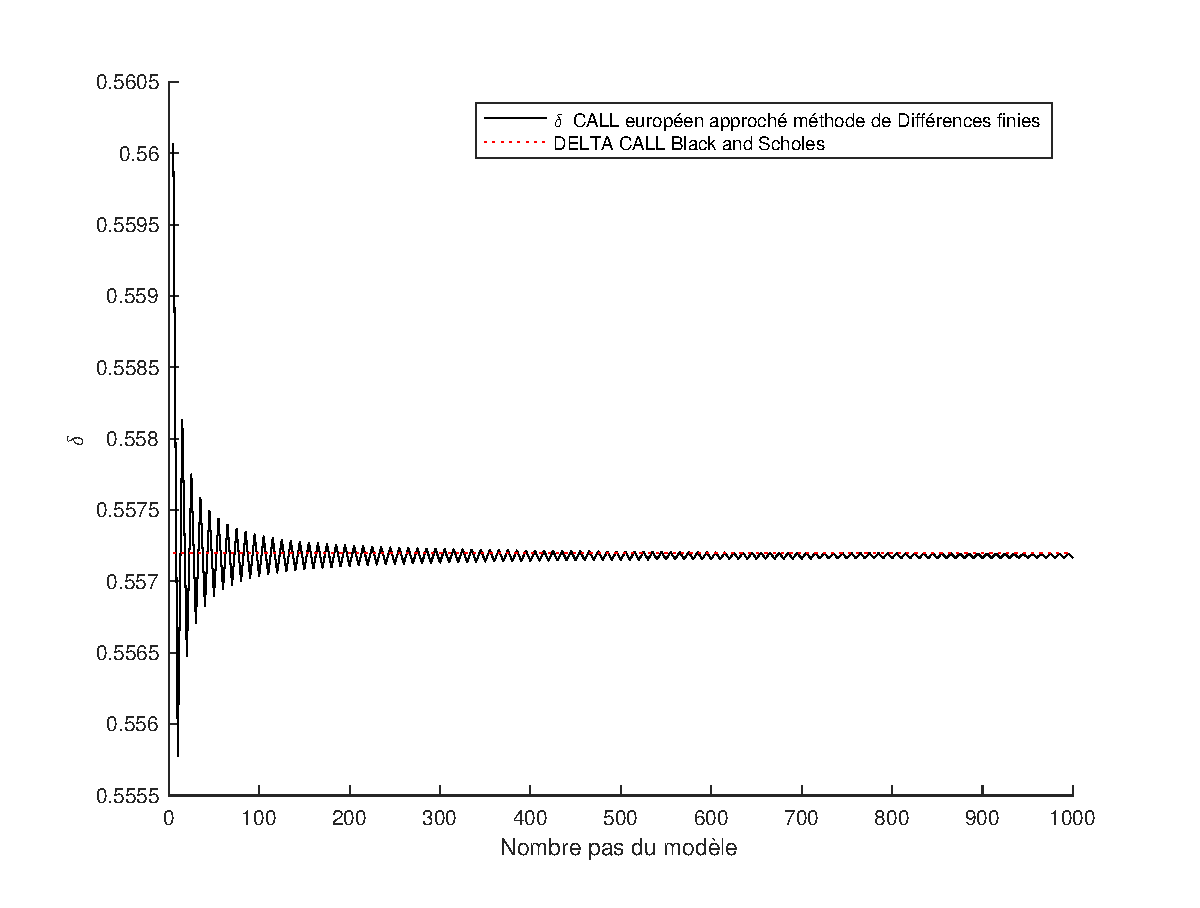
\includegraphics[scale=0.6]{./img/DELTA_CALL_EURO_DF-BS.eps}
\caption{Variation du $\delta$ d'un CALL européen approché par la méthode de différences finies en fonction du nombre de pas}
\label{fig:delta_call_euro_df}
\end{figure}

\begin{figure}[H]
\centering
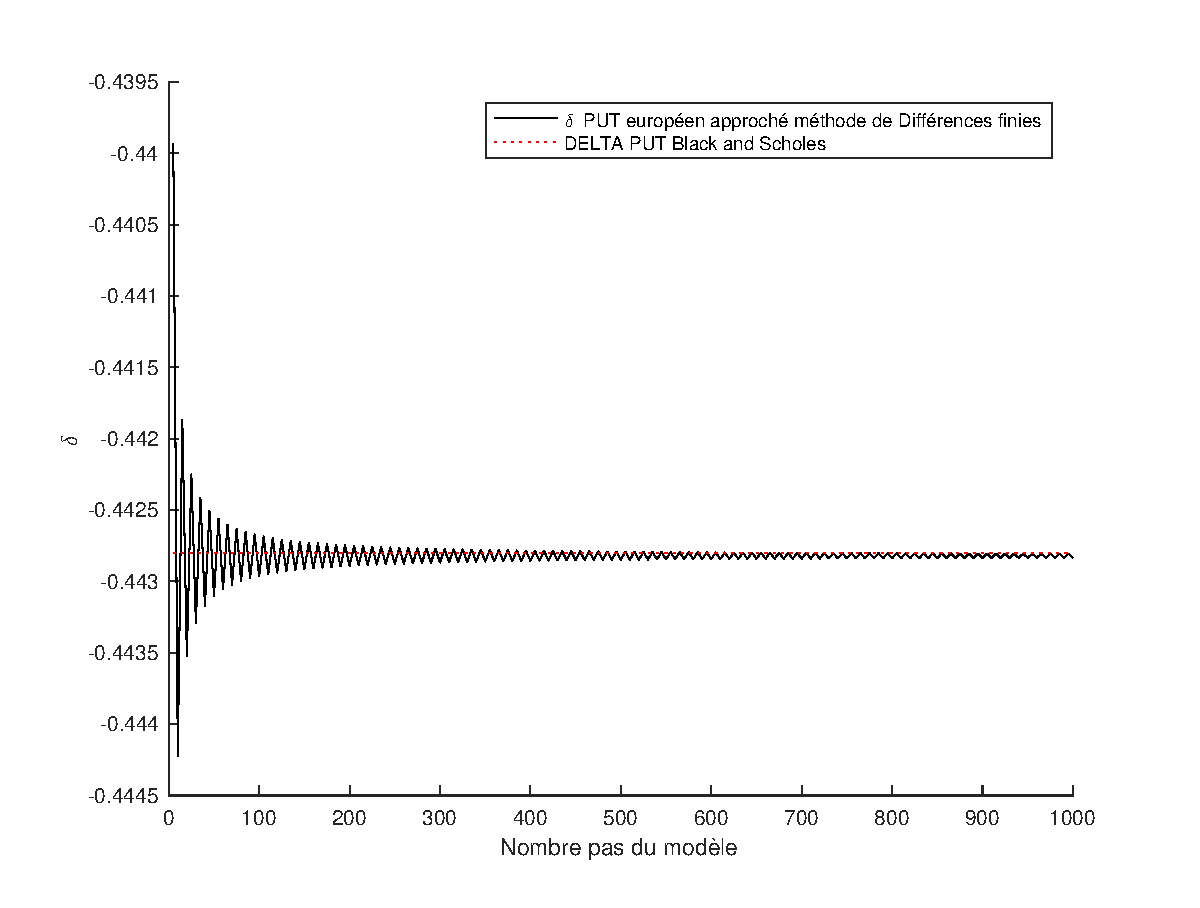
\includegraphics[scale=0.6]{./img/DELTA_PUT_EURO_DF-BS.eps}
\caption{Variation du $\delta$ d'un PUT européen approché par la méthode de différences finies en fonction du nombre de pas}
\label{fig:delta_put_euro_df}
\end{figure}

Il est clair que plus le nombre de pas augmente, plus l'amplitude de variation autour de $\delta$ diminue. De plus la vitesse de convergence est clairement rapide.

% section calcul_du_delta (end)

\newpage

\section{Monte-Carlo} % (fold)
\label{sec:question_5}

\section{Preguntas} % (fold)
\label{sec:preguntas}

\question{¿ Cuáles son los 4 tipos de valoración de impactos en evaluación ambiental ?}{
	\begin{itemize}
		\item Compatible: rápida recuperación sin medidas correctoras.
		\item Moderado: recuperación con tiempo pero sin medidas (medidas simples).
		\item Severo: recuperación con tiempo más medidas complejas.
		\item Crítico: recuperación supera el umbral tolerable y no es recuperable independientemente de las medidas que aplicamos.
	\end{itemize}
}

\question{¿ Funciones del coordinador de seguridad y salud en fase de proyecto y fase de obra ?}{
	\begin{itemize}[label=\ding{69}]
		\item Antes de la obra:
			\begin{itemize}[label=\ding{71}]
				\item  Aprobar plan de seguridad y salud elaborado por el contratista.
			\end{itemize}
		\item Durante la obra:
		\begin{itemize}[label=\ding{71}]
		 	\item Entrada con antelación suficiente para participar en decisiones técnicas.
		 	\item Verificación de protocolos.
		 	\item Control de acceso a obra (supervisión).
		 	\item Anotar en libro de incidencias.
		 \end{itemize} 
	\end{itemize}
}

\question{ ¿ Qué es un project manager ? Describe dos diferencias claves respecto a un director de obra.}{
	Es un gestor que controla el proyecto en su globalidad mediante el control de la calidad, el dinero y el tiempo. El director de obra tiene una misión más concreta: interpretar el proyecto y adaptarlo a la normativa vigente.
}

\question{¿ Cúales son las fases de un proyecto y en qué orden se realizan ?}{
	\begin{enumerate}
		\item Estudios previos
		\item Fase de concepción
		\item Fase de construcción
		\item Fase de explotación y mantenimiento
		\item Fase de cesión y/o desconstrucción
	\end{enumerate}
}

\question{ ¿ Quién realiza un proyecto ? }{
	\begin{itemize}
		\item Un consultor
		\item Una empresa de servicios 
		\item La organización promotora del proyecto
	\end{itemize}
}

% section preguntas (end)
% section question_4 (end)

\newpage

\section{Option barrière} % (fold)



Cette option s'annule  lorsque la barrière est franchie, elle est considerée comme exotique. Elle est une option plus sûre pour le vendeur car elle met une limite aux pertes potentiellement infinies sinon. Comme c'est une option plus risquée pour l'acheteur le prix de l'option est inférieur à celui d'une option vanille traditionelle. On la connait comme un CALL {\slshape up and out}. De plus on modelisera aussi un PUT avec barrière pour comprendre, comment implémenter la barrière et avoir une vision globale sur les 2 options. Le PUT avec barrière, aussi connu comme PUT {\slshape down and out} possède un barrière inférieure. On fera l'analyse avec une barrière à 65. Les Figure~\ref{fig:put_bar_payoff} et Figure~\ref{fig:call_bar_payoff} représentant le payoff de cette option en $t=T$ en fonction du cours du sous-jacent, $S_t$.

\begin{figure}[H]
\centering
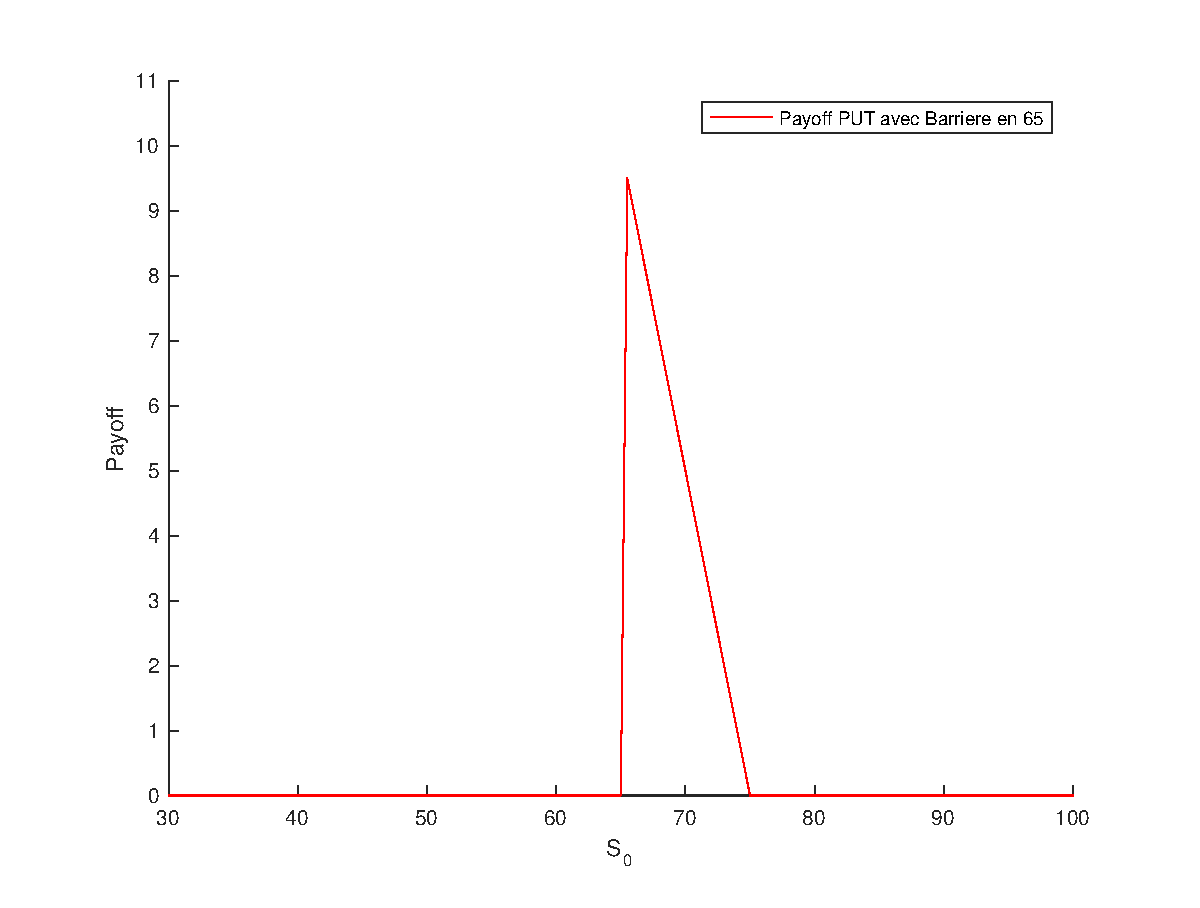
\includegraphics[scale=0.5]{./img/PUT_BAR_PAYOFF.eps}
\caption{Payoff d'une option barrière sur un PUT européen  en fonction du cours du sous-jacent}
\label{fig:put_bar_payoff}
\end{figure}

\begin{figure}[H]
\centering
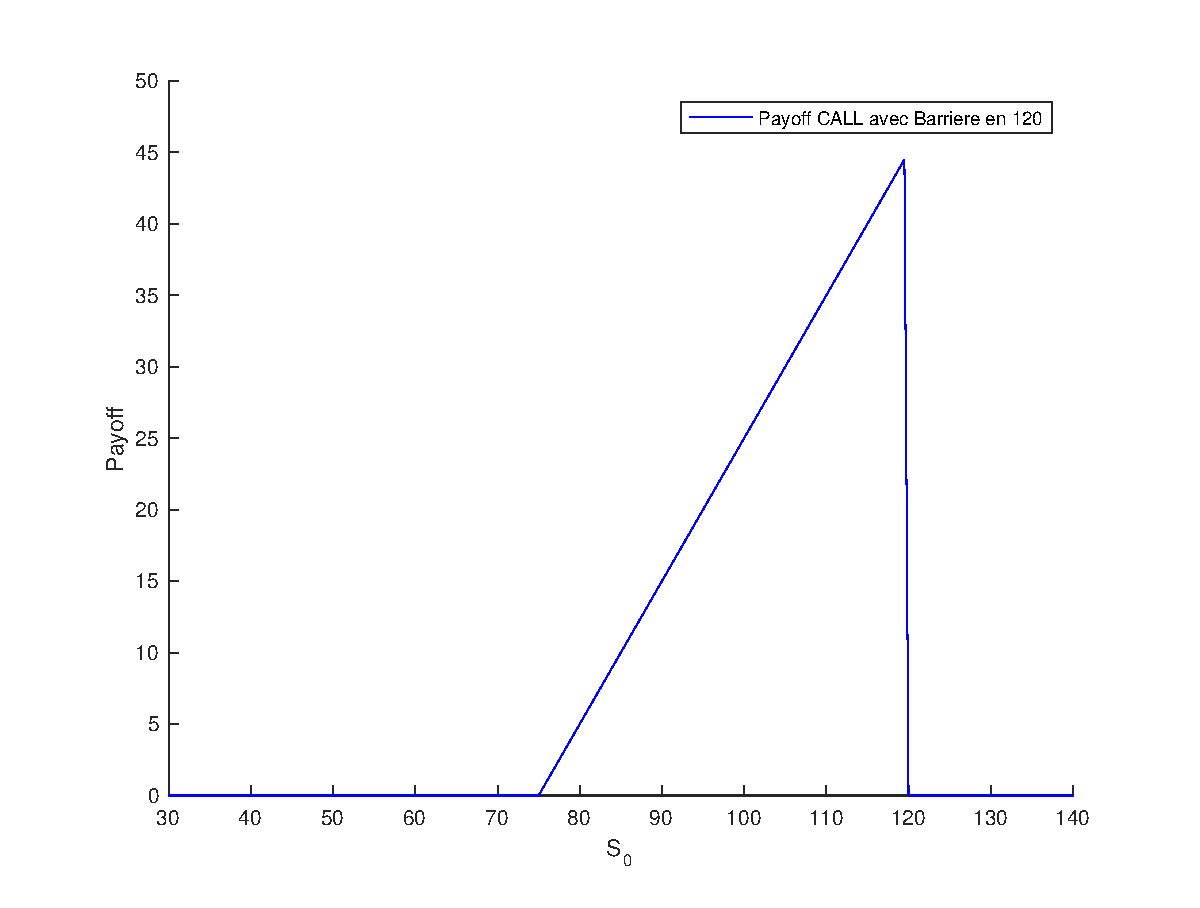
\includegraphics[scale=0.5]{./img/CALL_BAR_PAYOFF.eps}
\caption{Payoff d'une option barrière sur un CALL européen  en fonction du cours du sous-jacent}
\label{fig:call_bar_payoff}
\end{figure}

\subsection{Méthode de Monte-Carlo} % (fold)

\label{sub:methode_de_monte_carlo}

On analyse le prix de l'option en réalisant l'approximation de Monte-Carlo. La fonction pour le réaliser est Listing~\ref{listing:7}, le fichier dans lequel on la implémentée est \textsc{option$\_$barriere.py}. Les Figure~\ref{fig:call_put__bar_mc_tir}, Figure~\ref{fig:call_put_bar_mc} présentent les résultats obtenus.

\begin{figure}[H]
\centering
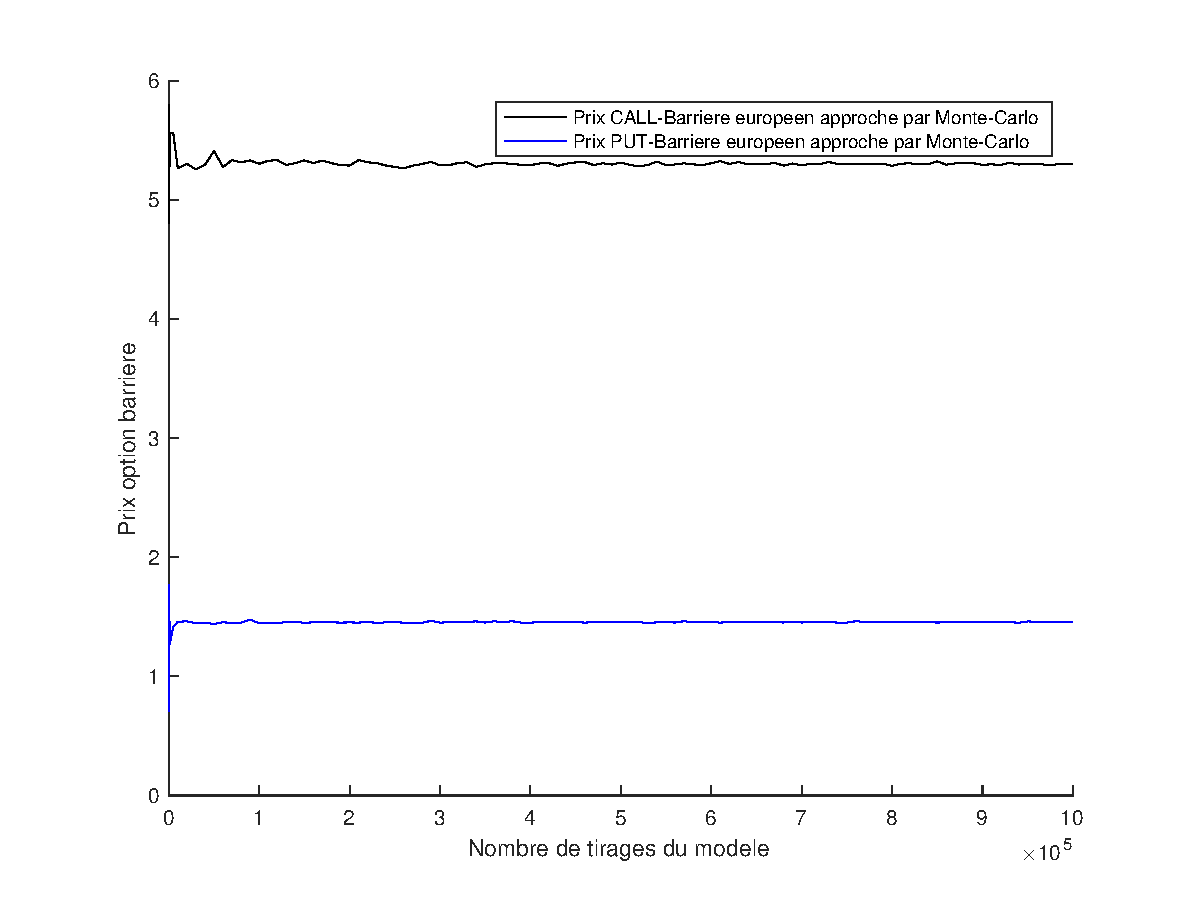
\includegraphics[scale=0.6]{./img/CALL_PUT_BAR_MC_TIR.eps}
\caption{Variation d'une option européenne avec option barrière approché par la méthode de Monte-Carlo en fonction du nombre de tirages}
\label{fig:call_put__bar_mc_tir}
\end{figure}

\begin{figure}[H]
\centering
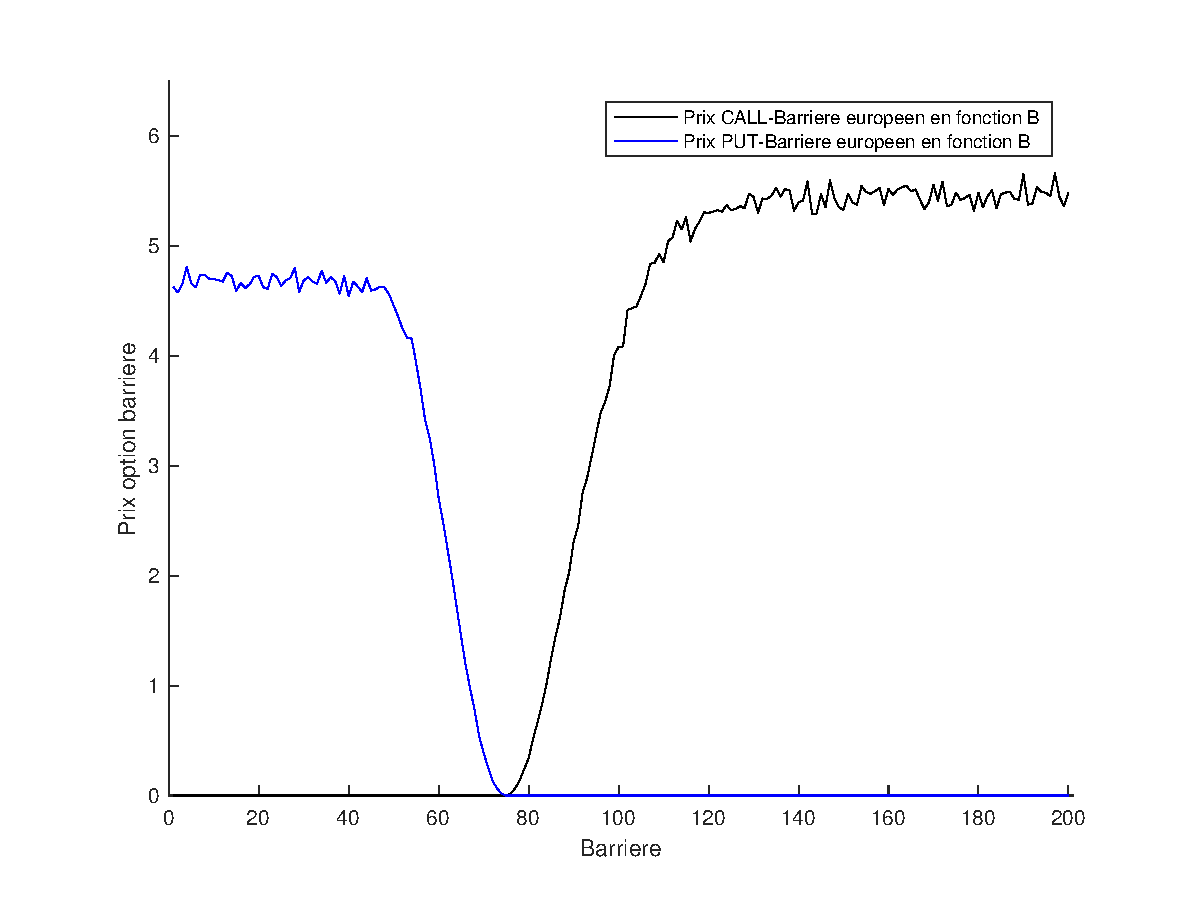
\includegraphics[scale=0.6]{./img/CALL_PUT_BAR.eps}
\caption{Variation d'une option européenne avec option barrière approché par la méthode de Monte-Carlo en fonction du niveau de la barrière}
\label{fig:call_put_bar_mc}
\end{figure}
% subsection methode_de_monte_carlo (end)

On peut voir que le prix du CALL augmente avec le niveau de la barriere et pour un barriere très grande, le prix est celui du modèle Black and Scholes. Pour le Put c'est exactement le contraire. Ce qui est logique, en effet si on pose la barrière très en dessous du prix \emph{At the Money} dans le cas d'un CALL, il est presque impossible que l'on ai un gain. Un raisonement similaire peut se faire pour le PUT.

On voit que le prix du PUT est inferieur au prix du CALL, car l'espérance de gain est inférieure.

\newpage

\subsection{Modèle Binomial} % (fold)
\label{sub:modele_binomial}

On analyse le prix de l'option dans le cadre du modèle binomial. La fonction pour le réaliser est Listing~\ref{listing:8}, le fichier dans lequel on la implémentée est \textsc{option$\_$barriere.py}. Les Figure~\ref{fig:call_put_bar_mb_prof}, Figure~\ref{fig:call_put_bar_mb} présentent les résultats obtenus.


Il est intéressant d'analyser comme sur la Figure~\ref{fig:call_put_bar_mb_prof} il y a plus de variations du PUT. La raison apparait sur la Figure~\ref{fig:call_put_bar_mb}, en effet on peut observer que pour un niveau de la barrière à 65, le delta du PUT est plus élevé que celui du CALL pour un niveau égal à 120.

\begin{figure}[H]
\centering
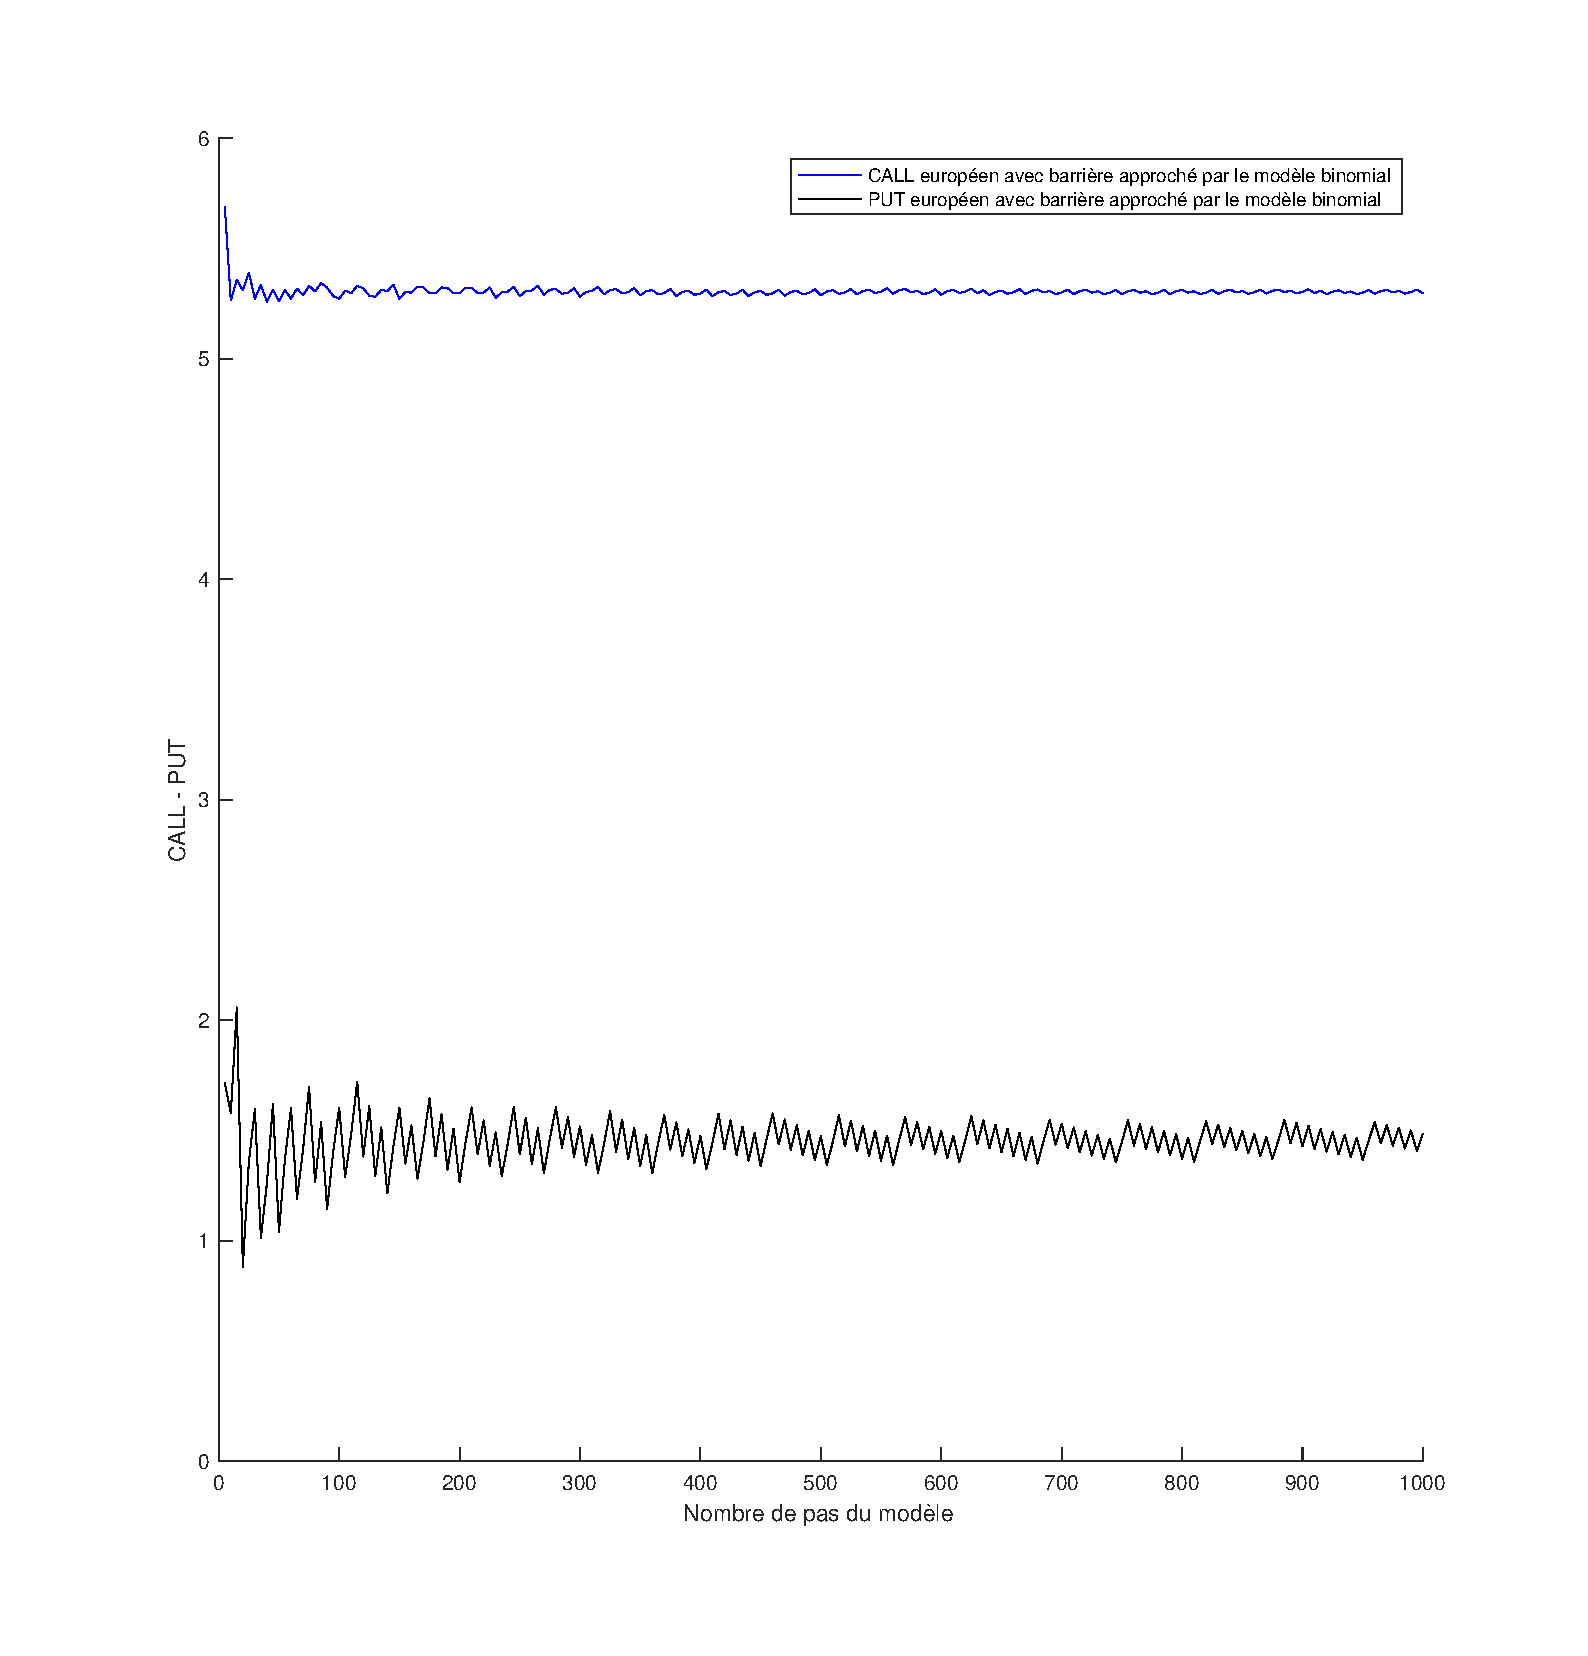
\includegraphics[scale=0.5]{./img/CALL_PUT_BAR_MB_PROFONDEUR.eps}
\caption{Variation d'une option européenne avec option barrière approché par le modèle binomial en fonction du pas}
\label{fig:call_put_bar_mb_prof}
\end{figure}

\begin{figure}[H]
\centering
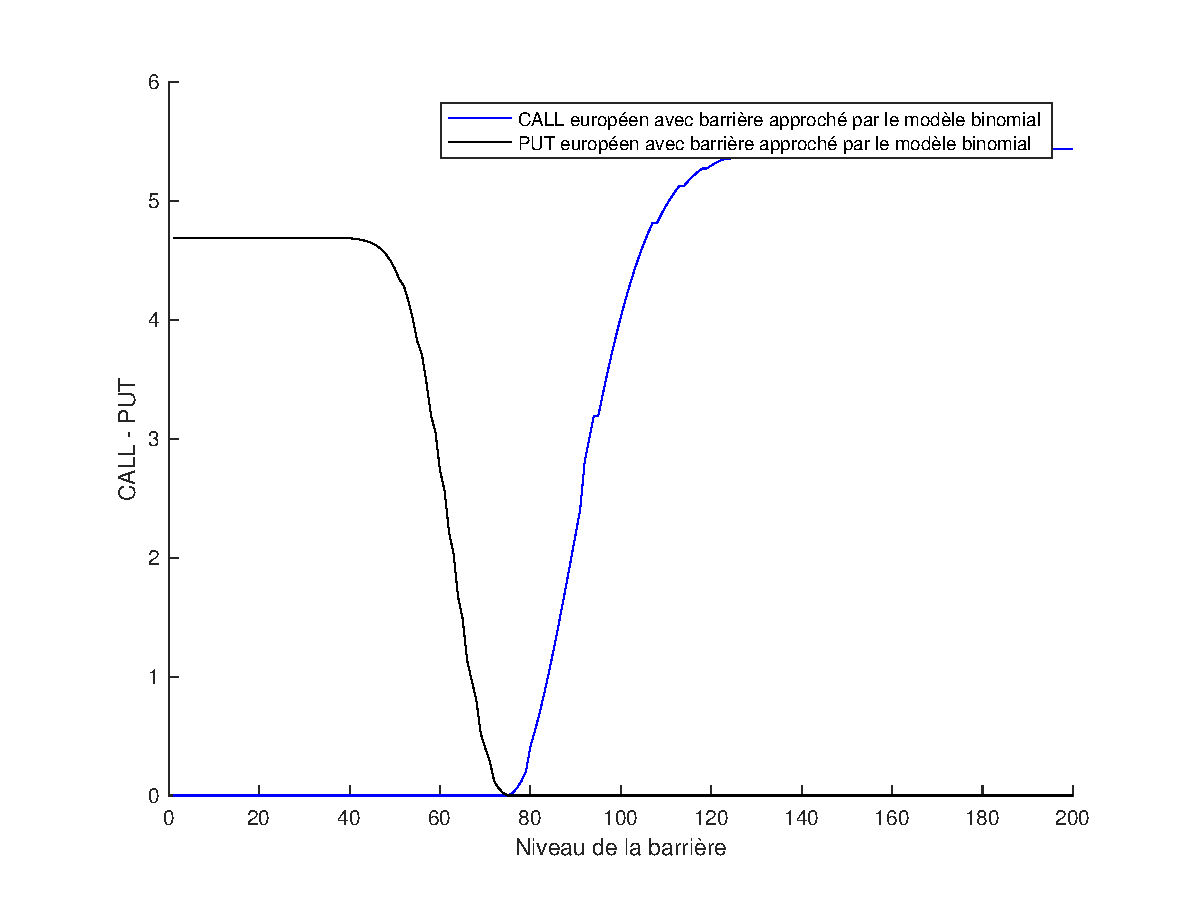
\includegraphics[scale=0.6]{./img/CALL_PUT_MB_BAR.eps}
\caption{Variation d'une option européenne avec option barrière approché par le modèle binomial en fonction du niveau de la barrière}
\label{fig:call_put_bar_mb}
\end{figure}

Les remarques sur les variations en fonction du PUT son les mêmes que dans le cadre Monte-Carlo. De plus on observe un lissage plus important, en effet la méthode de Monte-Carlo nécessite plus de tirages pour obtenir un résultat équivalent au modèle binomial. Cependant le grand avantage de la méthode de Monte-Carlo est que l'on n'a pas besoin de connaitre le modèle pour obtenir des résultats.

% subsection modele_binomial (end)

% section option_barriere (end)
\newpage

\section{Codes} % (fold)
\label{sec:codes}


\begin{listing}[H]
\inputminted[linenos,frame=leftline,breaklines=true,fontsize=\footnotesize]{matlab}{./codes/black_scholes.m}
\caption{Calcul du CALL et du PUT via la méthode de Black and Scholes. Matlab.}
\label{listing:10}
\end{listing}

\begin{listing}[H]
\inputminted[linenos,frame=leftline,breaklines=true,fontsize=\footnotesize]{matlab}{./codes/grecques.m}
\caption{Calcul des grecques du CALL dans le modèle de Black et Scholes}
\label{listing:11}
\end{listing}

\begin{listing}[H]
\inputminted[linenos,frame=leftline, breaklines=true,fontsize=\footnotesize]{python}{./codes/valeurs.py}
\caption{Fonction de calcul des valeurs nécessaires au modèle binomial}
\label{listing:1}
\end{listing}


\begin{listing}[H]
\inputminted[linenos,frame=leftline,breaklines=true,fontsize=\footnotesize]{python}{./codes/simul_arbre.py}
\caption{Simulation du payoff aleatoire dans le modèle binomial}
\label{listing:2}
\end{listing}


\begin{listing}[H]
\inputminted[linenos,frame=leftline,breaklines=true,fontsize=\footnotesize]{python}{./codes/modelebinomial.py}
\caption{Algorithme de calcul du prix d'une option via le modèle binomial}
\label{listing:3}
\end{listing}

\begin{listing}[H]
\inputminted[linenos,frame=leftline,breaklines=true,fontsize=\footnotesize]{python}{./codes/frontiere.py}
\caption{Calcul de la frontiere d'exercice d'une option americaine (temps,$S_t$)}
\label{listing:12}
\end{listing}


\begin{listing}[H]
\inputminted[linenos,frame=leftline,breaklines=true,fontsize=\footnotesize]{python}{./codes/delta_binomial_diff.py}
\caption{Algorithme de calcul du delta d'une option via le modèle binomial}
\label{listing:4}
\end{listing}

\begin{listing}[H]
\inputminted[linenos,frame=leftline,breaklines=true,fontsize=\footnotesize]{python}{./codes/montecarlo_bon.py}
\caption{Algorithme de calcul du prix d'une option europénne via la simulation de Monte-Carlo}
\label{listing:9}
\end{listing}

\begin{listing}[H]
\inputminted[linenos,frame=leftline,breaklines=true,fontsize=\footnotesize]{python}{./codes/delta_montecarlo.py}
\caption{Algorithme de calcul du delta d'une option europénne via la simulation de Monte-Carlo}
\label{listing:6}
\end{listing}

\begin{listing}[H]
\inputminted[linenos,frame=leftline,breaklines=true,fontsize=\footnotesize]{python}{./codes/option_bar_mc.py}
\caption{Algorithme de calcul du prix d'une option barrière via la simulation de Monte-Carlo}
\label{listing:7}
\end{listing}

\begin{listing}[H]
\inputminted[linenos,frame=leftline,breaklines=true,fontsize=\footnotesize]{python}{./codes/option_bar_mb.py}
\caption{Algorithme de calcul du prix d'une option barrière via le modèle binomial}
\label{listing:8}
\end{listing}

% section codes (end)

\end{document}